\chapter*{Introduzione}
\addcontentsline{toc}{section}{Introduzione}
Durante i primi anni di sviluppo del codice di Unix i programmatori cercavano di avere un codice ridotto e leggero, in modo che a runtime potesse richiedere meno risorse possibili e potesse essere ottimizzato per determinati scenari. Questo è causato dal fatto che in quegli anni le risorse erano limitate rispetto ai calcolatori di oggi e risparmiare anche pochi byte di memoria era cruciale al funzionamento del codice su un determinato processore. La tendenza è quella di ridurre al minimo i controlli, specie quelli di sicurezza, perché vengono considerati come ``overhead" e se ripetuti ad ogni ciclo di esecuzione, portano via preziose risorse come memoria e cicli di clock che potrebbero essere utilizzate per fare più calcoli e velocizzare l'esecuzione del programma. \\
\newline
Avere un numero ridotto di risorse è anche ciò che ha portato a sviluppare un'architettura come x86 a istruzioni variabili. Questo vuol dire che le istruzioni che devono essere eseguite sulla CPU sono variabili e solo della dimensione necessaria. In queto modo si possono risparmiare byte sullo stack e memoria durante l'esecuzione del programma. Questa implementazione porta con sé anche lati negativi e complica lo sviluppo dell'ISA che tende ad essere estesa più difficilmente avendo istruzioni di lunghezza diversa e non standardizzata. \\
\newline
Negli anni successivi questa architettura che è stata la base della maggioranza di processori sviluppati fino ad oggi, è stata ampliata all'esigenza, aggiungendo istruzioni, operandi e funzionalità. Nella pratica si tendeva ad aggiungere funzionalità sempre più complesse e che servivano a risolvere problemi specifici nell'architettura. Questa scelta è data anche dal fatto che aggiungere istruzioni nuove sarebbe stato meno costoso di implementare una nuova versione dell'ISA. Solo a causa di limiti fisici di memoria si è scelto di estendere l'architettura raddoppiando la lunghezza massima delle istruzioni e dei bit di indirizzamento. Infatti in un sistema che lavora a 32 bit è possibile indirizzare al massimo 4GB di indirizzi, che sarebbero quindi il limite massimo di memoria installabile in un sistema. Questo causerebbe un collo di bottiglia in caso si voglia estenedere verticalmente la capacità di calcolo di un calcolatore. Raddoppiando il numero di bit si può avere un limite teorico di 16 milioni di TB di spazio di indirizzi. L'esigenza di avere più indirizzi ha quindi fatto nascere la nuova architettura x86\_64 che è la base dei calcolatori odierni e si può trovare in processori di computer fissi, portatili e server. \\
\newline
Questo tipo di architettura è chiamata CISC (Complex Instruction Set Computer) ed è spesso paragonata alle architetture RISC (Reduced Instruction Set Computer) che offrono meno istruzioni, più semplici e di lunghezza fissa.\\
\newline
Nella figura \ref{fig:x86_64arch} è presente uno schema semplificato di una architettura x86\_64 che evidenzia le parti principali. Di questa porremo l'attenzione sui principali registri come RIP (Instruction Pointer Register) e sui registri a 64 bit.
\vspace{1cm}
\FloatBarrier
\begin{figure}[!htbp] 
    \centering
    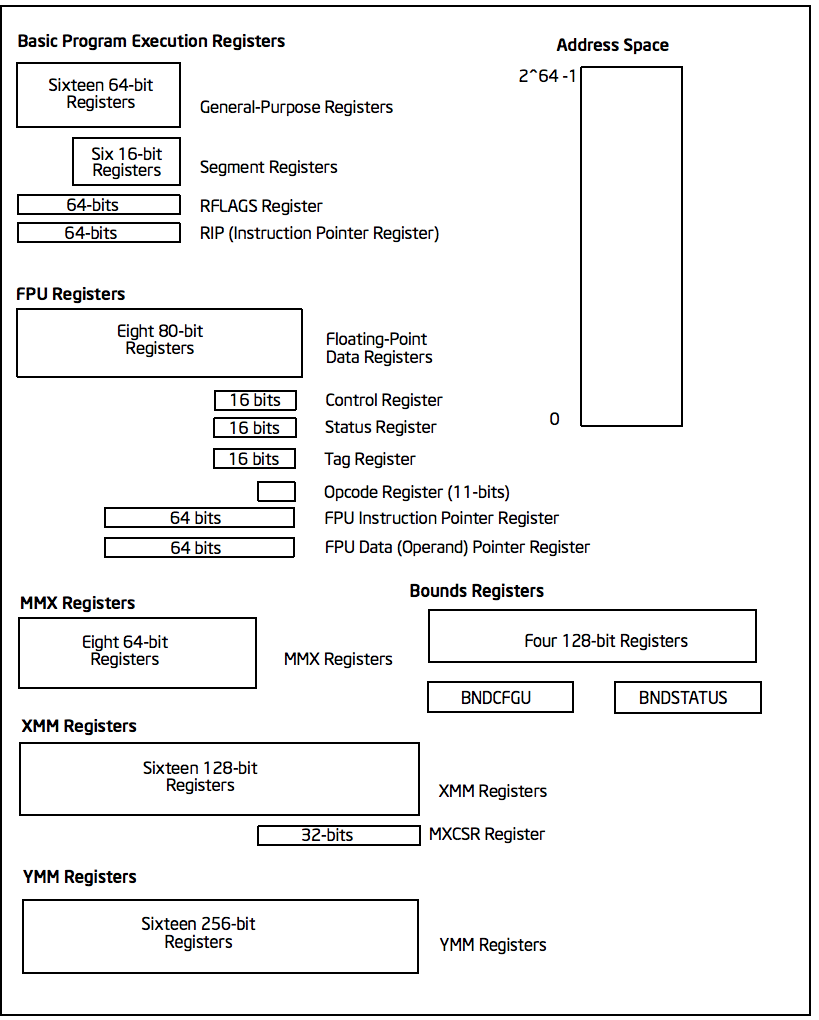
\includegraphics[scale=0.8]{images/x86-64-arch.png}
    \caption{Registri dell' architettura x86}
    \label{fig:x86_64arch}
\end{figure}
\FloatBarrier
\vspace{1cm}
Nelle architetture di tipo RISC abbiamo invece dei set di istruzioni ridotte, quindi meno istruzioni. Le architetture RISC anche per questa semplicità sono più facili da implementare. Oggi abbiamo ampio utilizzo di questo tipo di processori in dispositivi non-desktop, tranne pochi casi rari come i nuovi computer Apple Silicon \cite{Apple} di Apple. In genere, difatti, abbiamo processori RISC in dispositivi ``constraint" (ovvero con disponibilità poche risorse) come dispositivi IOT, Smartphone, sistemi embedded e system on a chip. Avendo un ISA open source è infatti possibile implementare l'architettura del calcolatore senza costi aggiuntivi e essendo facilmente implementabile è possibile creare microprocessori semplificati basati su queste architetture. \\
Nella figura sottostante è rappresentata una pipeline RISC-V a 5 stadi. È evidente la semplicità di un'architettura del genere, avendo un numero così ridotto di step (\textit{Fetch, ID, Execute, Memory e Write Back}). \\
Nonostante la semplicità implementativa, permette comunque di eseguire tutte le istruzioni che eseguirebbe un'architettura più complessa ed è completamente parallelizzabile.
\vspace{1cm}
\FloatBarrier
\begin{figure}[!htbp] 
    \centering
    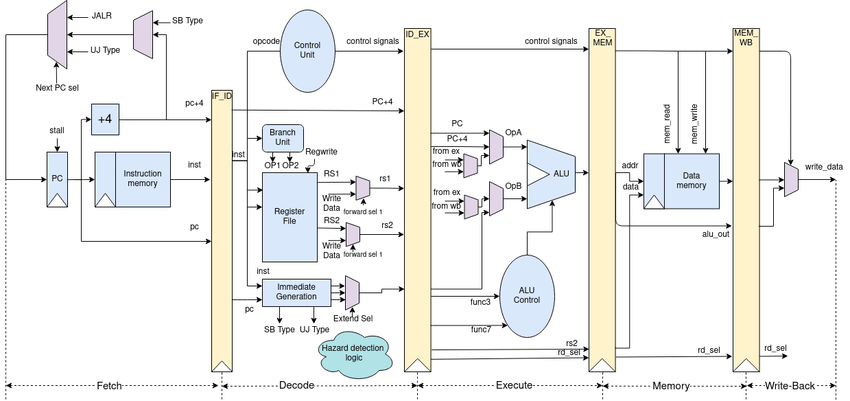
\includegraphics[width=1\linewidth]{images/risc-v-pipeline.png}
    \caption{RISC-V Pipeline}
\end{figure}
\vspace{1cm}
Date queste premesse, è chiaro che lo studio delle vulnerabilità e dei potenziali attacchi degli eseguibili prodotti da architetture moderne come quelle RISC è importante in un'ottica di hardening dell'infrastruttura. Lo studio delle path di exploit di queste architetture aiuta anche per capire quali sono i potenziali vettori di attacco che potrebbero esistere e che gli attaccanti potrebbero quindi sfruttare per manomettere eventuali sistemi ``constraint" basati su ISA RISC-V. \\
\newline
In questa tesi si analizzeranno le differenze tra le architetture per quanto riguarda gli eseguibili prodotti, le differenze di codice macchina, e si metterà a paragone anche la stessa tipologia di attacco sui due ambienti diversi, evidenziando l'efficacia in uno e nell'altro e le possibili mitigazioni.
\subsection*{Contributi}
\addcontentsline{toc}{subsection}{Contributi}
Il mio progetto si suddivide in due sezioni: una parte in cui verranno studiati attacchi alla memoria e una parte di analisi di attacchi side channel.\\
\newline
Nella prima sezione ho studiato gli attacchi Buffer Overflow e Return Oriented Programming su ISA RISC-V, paragonandoli agli stessi attacchi ma su architetture come x86 e x86\_64, evidenziando le differenze in termini di compilato, registri, codice macchina, indirizzi e difficoltà riscontrate.\\
In particolare, ho evidenziato un attacco basato su ``Data Oriented Programming" eseguito su RISC-V, che nello scenario in cui lo ho presentato, permette di manipolare il codice di uscita della systemcall \textit{exit()} senza utilizzare shellcoding o chaining di gadget, ma solo manipolando dati salvati nei registri dello stack.\\
Fornirò inoltre i compilati prodotti, in modo da poter essere analizzati in seguito da meccanismi di Control Flow Integrity. A scopo di test ho completato anche il porting dei programmi generati su piattaforma Cheshire.\\
Per concludere ho eseguito delle prove di generazione di ``ropchain" usando gadget estratti dal webserver NGINX compilato per RISC-V, per costruire un attacco Return Oriented Programming fornendosi di LLM.\\
\newline
Nella seconda sezione ho effettuato invece delle ``Proof of concept" di attacchi side channel e ho evidenziato in quali delle architetture testate sono efficaci.\\
\newline
Ogni codice, artefatto e test eseguito è tracciato nelle seguenti repository:\\
\begin{itemize}
    \item \href{https://github.com/BlessedRebuS/RISCV-Attacks}{\textbf{https://github.com/BlessedRebuS/RISCV-Attacks}}
    \item \href{https://github.com/BlessedRebuS/RISCV-ROP-Testbed}{\textbf{https://github.com/BlessedRebuS/RISCV-ROP-Testbed}}
\end{itemize}
\subsection*{Descrizione dei capitoli}
\addcontentsline{toc}{subsection}{Descrizione dei capitoli}
La tesi è suddivisa nelle seguenti macrosezioni. Nel \textbf{capitolo 1} vengono introdotte le tipologie di attacco alla memoria e vengono evidenziate le principali differenze tra attacchi su ISA RISC-V e x86 / x86\_64. Nel \textbf{capitolo 2} si elencano le tecnologie utilizzate e gli ambienti usati come ``testbed" di attacco. Nel \textbf{capitolo 3} vengono evidenziate le differenze tra le architetture in modo più dettagliato, con particolare attenzione sul linguaggio macchina e sui decompilati di alcuni programmi vulnerabili. Nel \textbf{capitolo 4} è presente la sezione in cui si elencano tutti i tipi di attacco effettuati, divisa in altre due sottosezioni: attacchi alla memoria e attacchi side channel. Nel \textbf{capitolo 5} sono esposte le conclusioni ed è presente la struttura delle repository in cui è possibile trovare i sorgenti del lavoro svolto.
\newpage